\chapter{Background}
\label{background}

\section{The OSS organisation}
Open-source and closed-source software projects have much in common on the
software level. However, on the organisational level, the two worlds differ a
lot.

The members of Free/Libre OSS (FLOSS) projects participate voluntarily as the
projects are open to everyone who wishes to contribute. In
closed-source/proprietary projects, contributors are selected by the management
through a hiring policy and salaries \cite{androutsellis}.

Decisions in OSS projects are mostly made by the core developers or project
leaders without a formal structure. Decisions can be made by a voting system. In
closed-source projects, the decisions are made by the organisational management
in a strict/rigid structure.

The releases in OSS projects are often done frequently, even minor improvements,
usually not on fixed dates. As opposed to closed-source software, with
infrequent major releases on fixed dates.

\paragraph{}
The differences as stated previously emphasise the fact that there is no
uniform and clear structure in OSS projects that enables the comparison of
multiple projects regarding activity and progress.

This organisation structure is also referred to as \textit{bazaar style},
because it is open for everyone to contribute \cite{androutsellis,
karus20132, nakakoji}. The bazaar style is the opposite of the
\textit{cathedral style}, where there is a group of elite members who decide
which contributions make it in the next release.


\section{Software evolution}
\label{section:lehman}
\subsection{Feedback loops}
The term \textit{software evolution} refers to the ever-going change a
software project goes through. This law of continuing change is the first of
the eight laws of software evolution by \citet{lehman}.

\citeauthor{lehman}'s laws are intrinsic to what he calls \textit{E-type}
systems \cite{lehman80}. E-type software systems ``\textit{\dots{}are programs
or applications that solve a problem or implement a computer application in the real
world.}''\cite{lehman}. This is the type of software that is taken under
analysis for this study.

\paragraph{}
Software does not evolve by intrinsic feedback loops, like evolution in plants
and animals, but by extrinsic feedback. Evolution by intrinsic feedback is
related to feedback pressures from within the organism. Software is not a
living organism and thus changes in the software are related to feedback
pressures from the outside world \cite{lehman}.

\paragraph{}
There is a need for continuing adaptation for E-type systems. The reason for
this is twofold: on the one hand there is the ever-changing requirements
and needs for the users of the software. People who use the software find bugs,
require more features, and so on. On the other hand there is the ever-changing
environment or world the software 'lives' in. If depending software is
changing, the change propagates to the system at hand.

Both types of extrinsic feedback result in changes of the original system and
'feeds' the evolution of the software.

\subsection{Maintaining complexity}
The extrinsic feedback is not the only source of change to a software system.
Continuously adapting to environmental and users' needs eventually pays its
toll. As the second law of \citeauthor{lehman} says that ``\textit{\dots{}as a
software project is evolving, the complexity of the program increases unless
work is done to maintain or reduce it}'' \cite{lehman}. This means that, due
to changing the software as a result of changing needs in the environment or
users, the software needs to change even more in order to keep it below a
certain level of complexity.

\subsection{Activity}
The fourth law of software evolution by \citet{lehman} -- the law of
organisational stability -- denotes that the ``\textit{\dots{}average effective
global activity rate on an evolving system is invariant over the product life
time.}''.

The most interesting finding of \citeauthor{lehman} in this law is that the
invariance holds regardless of managerial decisions. This means that the
activity of a healthy software system is constant over the life time of the
product.

\paragraph{}
\citeauthor{lehman}'s laws of software evolution are valid for both closed
source software and open-source software. These laws form the foundation of
what we understand as software evolution.

\paragraph{}
The evolution of a software system comprises various measures on different
moments in time. For instance, the lines of code metric over a project's life
time is a way to measure the evolution of lines of code in a software project.
More on the measures of software evolution in the next sections.





\section{Success factors}
In the survey of OSS projects by \citet{androutsellis}, project success is
defined from three perspectives:

\begin{description}
	\item[Prerequisites for success] \hfill \\ The prerequisites for a good
		chance of a successful project are divided in four categories: the first is
		the need for \textit{starting points} for a project. The starting points
		are threefold; (1) a certain interest is required in the mind of one person
		or a group of developers; (2) the audience the software is targeting
		should be clear from the beginning; and (3) the natural language of the
		project may play an important role.
		
		Second is the \textit{community organisation}. A meritocratic culture would
		be the best chance for a successful project. That is, a culture that is ruled
		by the people who deserve it. The leaders come from the inside of the
		community and are by definition supported by that community.
		
		Third is the aspects that contribute to the prerequisites for success are the
		\textit{technical} environment and infrastructure as well as programming
		language. This contributes to the efficiency of the software development
		process. The choice of external project dependencies affects the success of a
		project under development.
		
		And fourth, a prerequisite for project success is the \textit{open-source
		perspective}. The licensing scheme and the definition of an effective and
		reasonable business model are issues that should be clear from the beginning
		of a project.
		
	\item[Sustainability] \hfill \\ Ensuring the sustainability of a project
		that has reached a certain level of success. At the system level this means
		achieving identified goals, update documentation and testing material. The
		importance of software maintainability plays an important role in the
		sustainability of a successful project. This shows similarities to the second
		law of \citeauthor{lehman}'s laws of software evolution \cite{lehman}.
		
		On the community level, sustainability is evenly important. This comprises the
		level of developer and user satisfaction. This can be achieved through
		continuously evolving and taking advantage of the developers' skills and
		competencies \cite{androutsellis}.

	\item[Indicators for success] \hfill \\ The indicators to distinguish a
		successful project from other, less successful ones are of interest by
		many researchers. A lot of indicators for success or success factors have
		been identified, but the ultimate key indicators for success have not yet
		been found. The next section will elaborate more on this subject.
\end{description}

\subsection{Indicators of success}
Success is not a binary state but requires a measurement; a certain extent of
prosperity.

\paragraph{}
The survey by \citet{androutsellis} identified success indicators in four
perspectives. A project that has progressed into advanced development stages is
more likely to be a healthy project. Such projects have an active community of
developers.

The number of downloads is an indicator for success; a frequently downloaded
project is likely to be successful.

Frequent and visible development or bug fixing activities are indicators of a
healthy and successful project.

Another indicator for project success is the robustness of a project. Indicators
for a robust project are also indicators of success, according to
\citet{androutsellis}.

\paragraph{}
\citet{delone1992} defined a model of information systems success (Figure
\ref{figure:dm1992}). In this model, success factors are identified on multiple
levels: system and information quality, use and user satisfaction, and
individual and organisational impact. In the revised article \cite{delone2003}
the authors evaluate the model using more recent empirical results on the
application of their model across different studies.

\begin{figure}[H]
\caption{The Delone \& McLean model of information system
success (1992)}\label{figure:dm1992}
\caption*{\\[1em]}
\centering
	\fbox{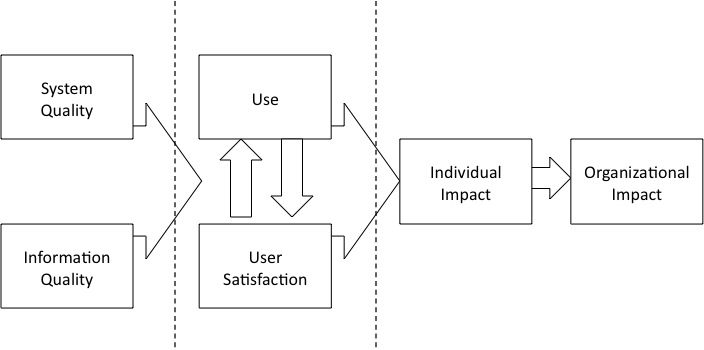
\includegraphics[scale=0.5]{images/DM1992.jpg}}
	\caption*{\footnotesize\textit{\copyright{1992} \citet{delone1992}}}
\end{figure}

\paragraph{}
It was found in between four and sixteen studies that there are significant
relations between ``system use'', ``system quality'', and ``information
quality'' on the one hand, and ``individual impacts'' on the other hand.

\begin{description}
	\item[System use] was typically voluntary in sixteen studies and measured as
		frequency of use, time of use, number of accesses, usage pattern, and
		dependency.

	\item[System quality] was measured in five studies in terms of ease-of-use,
		functionality, reliability, flexibility, data quality, portability,
		integration, and performance.

	\item[Information quality] was measured in four studies as accuracy,
		timeliness, completeness, relevance, and consistency.

	\item[Individual impact] was measured in terms of job performance,
		decision-making performance, job effectiveness, and quality of work and work
		environment.
\end{description}

\paragraph{}
A study by \citet{crowston2003} took the idea of \citeauthor{delone2003}
\cite{delone1992, delone2003} and examined the vision of system development
underlying the model and project them onto OSS projects. The authors identified
additional measures that might be used for OSS project success. The vision is a
process model that has just three components: the creation of a system, the use
of the system, and the consequences of the system use.

\citet{crowston2003} suggest that given the large number of abandoned projects,
the completion of a project is an indicator for success. However, it is hard to
define what it means for a project to be completed. Therefore, the progress of
a project from one development stage to the other is considered an indicator for
success. This is similar to the findings of \citet{androutsellis}.

Another indicator for success is whether the project achieved its goals. The
problem is that OSS projects often do not express their goals and do not have
formal requirement specifications. One goal that is often implicit in OSS
projects is developer satisfaction. This, in turn, is similar to findings of
\citet{androutsellis}.

\paragraph{}
Measures regarding the process of software development are identified.
\citet{crowston2003} states in accordance to \citet{lehman} that
software development is an ever-going activity. A number of possible indicators
of success are suggested by \citeauthor{crowston2003}:

\begin{description}
	\item[Number of developers] \hfill \\ The number of developers appears
		important for the continuity of a project and could therefore be an indicator
		of success.

	\item[Level of activity] \hfill \\ Seems to be more important than the number
		of developers. The developers' contribution to the project in submitting code,
		and bug reports.

	\item[Cycle time] \hfill \\ The time between releases, or cycle time, might
		be an indicator for success. The norm of the OSS community in general is
		'release early and often', which implies an active release cycle is a sign of
		a healthy project.

	\item[Employment opportunities] \hfill \\ The motivation of OSS developers
		might be an indicator for success. Developers may participate in an OSS
		project to improve their employment opportunities. It can be measured as
		their salary, or jobs acquired.

	\item[Individual reputation] \hfill \\ Related but not quite the same as
		the employment opportunities it is considered an indicator of success if
		developers are willing to participate because they will be rewarded with
		reputation in the community. Measurement, however, is very difficult. Earlier
		studies did not succeed in relating the earning of reputation to the
		success of a particular project.

	\item[Knowledge creation] \hfill \\ An effect that can be measured by
		surveying the developers for their perceived learning on a project. It seems
		important for developers that they learn during their participation in a
		project.
\end{description}

\noindent
Although important, the previous list of measures is by no means an exhaustive
list of measures for OSS project success. The disclaimer by \citet{crowston2003}
states that by no means they claim that any of these measures actually measures
project success.

\paragraph{}
In another study, three years later, conducted by \citet{crowston2006}, the
authors extended the earlier study using Free/Libre Open-Source Software (FLOSS)
projects. The authors demonstrated the application of the measures as listed in
the previous paragraphs in 122 projects from
SourceForge\footnote{\url{http://www.sourceforge.net}}.
The paper shows the challenges for mining source code repositories and OSS communities.

One measure that was revisited is the \textit{number of developers}.
\citeauthor{crowston2006} suggests the 'number of developers' as a measure is a
flawed number, because it aggregates the numbers of developers joining and the
leaving a project. A developers 'churn' (i.e., sum of developers joined and
left) or a 'tenure' (i.e., developers time on the project) would be more
appropriate in measuring team size or composition.





\section{Evolution in OSS}
\subsection{Project transition}
A research by \citet{nakakoji} studied the 'natural product evolution' of OSS
projects using four typical OSS projects. Three categories of software were
identified:

\begin{description}
	\item[Exploration-oriented] \hfill \\ Sharing innovations and knowledge.
	\item[Utility-oriented] \hfill \\ Satisfying an individual need.
	\item[Service-oriented] \hfill \\ Providing a stable service.
\end{description}

\noindent
\citeauthor{nakakoji} found that the community of an OSS project co-evolves
with the system. Additionally the authors found that OSS projects evolve from
one category to the other. Typically, an exploration-oriented project evolves
into a service-oriented project. A successful exploration-oriented project
attracts many developers which speeds the code evolution, mostly not in favour
of the exploration-oriented project goals. This increases the risk of the
project to be forked and the original project to be abandoned.

Utility-oriented projects also typically mutate into service-oriented projects.
According to \citeauthor{nakakoji} the service-oriented variant of a utility is
a merge of combined forces of multiple utility-oriented projects providing
similar features.

\subsection{Project characteristics}
A study by \citet{koch2007} analysed the evolution of more than 8,621 OSS
projects from SourceForge. The projects are analysed by the following metrics:

\begin{description}
	\item[Lines of code (LOC)] \hfill \\ At the initial commit of a project,
		the LOC is computed for all source files. For any subsequent commits, the LOC
		added, and LOC deleted is recorded. The difference between LOC added and
		deleted can be used to compute the cumulative LOC at any given time.

	\item[Revision] \hfill \\ The submission of a single file by a single
		programmer.
		
	\item[Maturity] \hfill \\ An indicator of maturity is given by SourceForge
		ranging in seven possible values: planning, pre-alpha, alpha, beta,
		production/stable, mature, and inactive. This metric is equal to the
		development stage indicator of \citet{androutsellis} and
		\citet{crowston2006}.
\end{description}

\noindent
The projects are analysed by the previously mentioned metrics. Findings of the
analysis are mostly done on growth characteristics. A result was that a higher
number of active programmers has no negative influence on productivity in mean
output per programmer in LOC. The same counts for output per programmer in
revisions.

Furthermore, it was found that projects with super-linear growth are larger in
LOC, are more active in number of revisions, and have more programmers, than
projects with linear growth. However, the previous findings do not always count
for super-linear versus sub-linear growth.

\paragraph{}
A study conducted by \citet{beecher} on the characteristics of a total of
300 FLOSS projects from 6 distinct repositories used metrics to measure
and characterise the projects, similar to \citet{koch2007}.

One additional metric was used by \citeauthor{beecher} in comparison to the
other studies:
\begin{description}
	\item[Duration] \hfill \\ Measured as the number of days over which the
		project was developed. This was evaluated using the earliest and latest
		available dates in the source code repository for the project. It gives the
		actual age of the project, at least since the moment the community decided to
		use a source code management system. It is a good indicator of the time-span
		of the project.
\end{description}

\noindent
It was found by \citeauthor{beecher} that repositories differ from each other in
terms of product and process characteristics. The authors compared two groups of
projects characterised by repository. The first group having projects from
Debian, KDE, and GNOME, and the second from RubyForge, Savannah, and
SourceForge. Both groups show consistently different characteristics in size,
duration, commits, and committers. These metrics were used to identify success
relative to other projects in the same group and across groups. A growth in
size, a relatively longer duration, relatively more commits and committers
would be 'more successful'.

\citeauthor{beecher} found that the projects in the first group achieve better
results compared to the second group. Projects that made the transition from
the second to the first did better on previous metrics than before the
transition. This implies that the type of repository influences the project
success. Projects in repositories Debian, KDE, and GNOME are in general more
successful than projects in repositories RubyForge, Savannah, and SourceForge.
This is probably due to the stricter rules for a project to enter one of the
repositories in the first group and the free nature of the repositories in the
second group.



\subsection{Software evolution prediction}
A study by \citet{goulao} used seasonal time analysis to predict the evolution
of OSS projects. The authors use an ARIMA\footnote{auto-regressive integrated
moving average} model that fits time series data (i.e., a sequence of data
points measured at successive, uniformly spaced data points) of change
requests.

The findings of \citeauthor{goulao} were that not all projects show seasonal
patterns. The ARIMA model was trained on one project's history data (in this
case, Eclipse) to be able to accurately predict the evolution of that project.
After training, the model could actually adequately predict evolution in the
long-term.

Although, the prediction of evolution using the ARIMA model is not subject to
this study, but it does show that the predictability of the evolution of OSS
projects exist.



\section{Project survivability}
Several studies have been conducted regarding the survivability of OSS projects
\cite{raja2012, samoladas2010, wang2012}.

\paragraph{}
\citet{raja2012} defined and evaluated a measure of survivability of OSS
projects. The measure the authors found is \textit{viability}: \textit{the
ability of a project to grow and maintain its structure in the presence of
perturbations}. The viability is defined along three dimensions:

\begin{description}
	\item[Vigor] \hfill \\ The ability of a project to grow/evolve over a period of
		time. Measured as number of versions released per year.

	\item[Resilience] \hfill \\ The ability of a project to recover from
		disturbances. Measured as response time to artifact requests.

	\item[Organisation] \hfill \\ The structure exhibited in the project. Measured
		as average mutual information. That is, the structure of the artifact
		management process reflects the organisation of the project.
\end{description}

\noindent
The viability of a project was tested in 232 random projects from SourceForge,
of which 136 projects were used as analysis sample, and 96 as validation
sample.

The three dimensions are mathematically formulated to compute a coefficient
representing the 'value' of either of the dimensions. A higher value indicates
a stronger position in the dimension.

The authors found that viability is consistent with reality. In addition, the
three dimensions -- vigor, resilience, and organisation -- are different
attributes contributing to viability.

\paragraph{}
In a study by \citet{samoladas2010} on the survivability of OSS projects,
the authors performed an analysis on the duration of 1,147 OSS projects from
various sources using a similar, but slightly different, interpretation of the
duration metric of \citet{beecher}:

\begin{description}
	\item[Duration] \hfill \\ The age of the project in months since the birth
		month (i.e., the first month the project was present in the data). Projects
		are split into two groups: the active, and inactive projects. Inactive
		projects have had less than two commits for two months in a row.
\end{description}

\noindent
\citeauthor{samoladas2010} employed a Kaplan-Meier estimation of the survival
function and the hazard function of the projects. Analysis was performed by
using the duration metric on all projects, and on projects category as the
projects were categorised in 25 distinct categories.

The findings by \citeauthor{samoladas2010} were that there is an effect of
project category (i.e., application domain), and number of committers on the
duration of a project. For instance, adding developers to a project increases
the survivability of a project. The authors proposed two main research issues to
be addressed in the future. The first is to add more projects to the study with
possibly a different categorisation as it may influence the results. And second,
the effects of more project parameters, such as programming language should be
examined. This is not trivial since typical more than one language is used in a
project.

\paragraph{}
\citet{wang2012} investigated survival factors of FLOSS projects obtained from
SourceForge. \citeauthor{wang2012} conducted the investigation at two stages
of a project's life cycle. These stages are:

\begin{description}
	\item[Initial stage] \hfill \\ The initial period of time, typically the first
		year of existence when there is no public release of source code.
	
	\item[Growth stage] \hfill \\ The period of time after the first public release
		of the core source code, typically after the first year of existence.
\end{description}

\noindent
\citeauthor{wang2012} defined the following independent variables and
measures for OSS project survivability:

\begin{description}
	\item[Survival in initial stage] \hfill \\ The likelihood of a project to
		survive the first year. Measured by the ability to remain active on hosting
		website.

	\item[Survival in growth stage] \hfill \\ The likelihood of a project to
		survive after the first year. Measured by the ability to produce the first
		release of source code, adoption rate, and technical improvements.

	\item[User/developer participation] \hfill \\ The extent to which
		users/developers are involved in the development of the software. Measured by
		involvement of users and developers in bug submissions, bug fixes, etc.

	\item[Service quality] \hfill \\ The degree to which the project team satisfies
		the needs and requirements of the users and developers. Measured by the
		implementations of feature requests, bug fixes, and the degree to which users'
		needs are satisfied.

	\item[License restrictiveness] \hfill \\ The degree of restrictions on the
		users and developers to redistribute software derived or modified from the
		project. Measured by the classification of the OSS license type of the
		project.

	\item[Targeted users] \hfill \\ Whether a project is targeted at technical
		users. Measured by the targeted user group; whether the user group is software
		developers or systems administrators.

	\item[Internal network size] \hfill \\ The size of the network of developers
		from within the project, measured by the number of developers.

	\item[External network size] \hfill \\ The number of members and members of
		other OSS projects that developers of the project are involved with.

	\item[Quality of external network] \hfill \\ Measured by the SourceForge
		ranking of the affiliated projects.
\end{description}

\noindent
The findings of \citet{wang2012} were that the level of OSS projects'
user/developer participation will positively impact the project's survival at
initial stage. However, it is only marginally supported that the same holds for
the project's survival at growth stage.

The level of service quality will positively impact the project's survival at
both the initial and growth stages. The license restrictiveness has no
significant impact on the survivability of a project. This is in contrast to
the observations regarding open-source perspective of \citet{androutsellis}.

Furthermore, network sizes do not impact the survivability, but the quality of
the external network does at both stages.

\paragraph{}
\citet{wang2012} also found that warning indicators can be found in six factors
of OSS project success: developer participation effort, developer service
quality, license restrictiveness, targeted users, external network size, and
external network quality. A decay in one or more of these factors might be a
warning sign.

\subsection{Project causes of death}
According to \citet{karus20132} there can be two reasons for an OSS project to
die:

\begin{description}
	\item[Loss of popularity] \hfill \\ A product loses its share because of
		other similar projects. Or a project has lost its value because of technical
		advances on other platforms, or deprecated hardware/software dependencies.
		
	\item[Reaching maturity] \hfill \\ A project might reach maturity in case it
		will be used without changes for the foreseeable future.
\end{description}

\noindent
The second of the two reasons is in contrast with \citet{lehman}'s laws of
software evolution as noted in section \ref{section:lehman}.

Besides the previous two reasons, one more reason can be thought of using the
study by \citet{nakakoji}. The \textit{forking} of a project, i.e., starting
a new project from an existing one. The two projects become substitutes and
eventually one will replace the other. Both projects evolve separately.

The effect of these events will ultimately result in \textit{abandonment} by
the developers, the users, and the entire community.

\paragraph{}
Detecting such events and 'predicting' the end of code evolution of OSS projects
is the subject of this study. One proposed method to accomplish this is using
wavelet analysis on evolution signals of OSS projects.



\section{Wavelet analysis}
\label{wavelet_analysis}
\citeauthor{karus2013} explored a method known as \textit{wavelet analysis} to
analyse software evolution data \cite{karus2013, karus20132}. The wavelet
analysis interprets evolution data as a series of signals and is able to find
sequences in this signal. The sequences of multiple projects can be compared in
order to find recurring patterns.

\paragraph{}
A study by \citet{hindle} explored the use of Fourier transform and analysis to
find repeating patterns or processes hidden in the logs of change events of OSS
projects. However, Fourier transform seems not the right tool to use for
analysis of evolution time series data.

\paragraph{}
Wavelet analysis is similar to Fourier analysis with the difference that
wavelet transform deals with time and frequency information, and Fourier
transform deals with frequency information only. Wavelet analysis has the
advantage over Fourier analysis that it can deal with non-smooth ('choppy')
signals, as opposed to the limitation of only sines and cosines \cite{graps}.

\subsection{Waveforms and wavelets}
Wavelets are functions that satisfy certain mathematical requirements and are
used in representing data or other functions \cite{graps}.

A waveform, or wave, is a signal (time-series) in a two-dimensional space.
Waveforms are used to model many types of signals, such as audio,
electromagnetic (light), gravitational, and quantum mechanical waves.

\paragraph{}
In many models of waveforms the two dimensions typically represent the time and
frequency domains. An audio signal is an example of a waveform modeled that way.

In visualisations of waveforms, the time domain is often plotted on the
horizontal axis, and the frequency domain on the vertical axis. In the example
of an audio wave (see Figure \ref{figure:wave}), the frequency domain may
represent the amplitude, or the frequency, and the time the duration of the
amplitude or frequency value.

\begin{figure}[h]
\caption{Example of an audio wave}\label{figure:wave}
\centering
	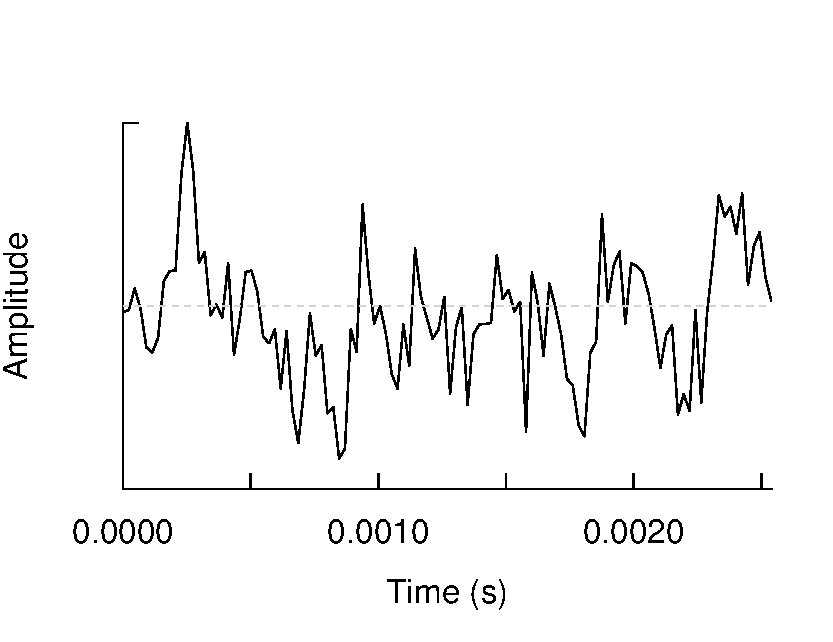
\includegraphics[height=192pt]{images/pink_audio.pdf}
\end{figure}

However, the time domain is not specifically bound to time intervals only. A
less intuitive approach could be to model frequency in the time domain. That
way the frequency relation to amplitude of a signal can be analysed, but the
time information is lost.

\subsection{Discrete wavelet transform}
To be able to analyse and compare wavelets of different lengths and scales, a
way to transform the signal is needed. Discrete wavelet transformation is the
operation of applying a filter function, or set of filter functions (also known
as 'filter bank') to the wavelet. 'Discrete' because the signal is segmented
into samples; which number is possibly finite, possibly infinite. The
discrete wavelet transformation is a way of sampling the signal at different
intervals giving a natural means of scaling the signal \cite{karus2013}.

\paragraph{}
In digital signal processing, the category of methods that discrete wavelet
transform belongs to, there is a phenomenon called the \textit{uncertainty
principle}. It means that the shorter the signal, the harder it is to
identify the signal. On the contrary, the longer the signal, the higher the
accuracy in identifying the signal. However, it is impossible to identify a
signal with 100\% accuracy as there is always a degree of uncertainty in
identifying a signal. This is a fundamental principle in digital signal
processing and it highly influences the ways the method can be used.

High-frequency signals vary quickly and are shorter in nature than
low-frequency signals that vary slowly. Therefore, in order to identify
high-frequency signals, time resolution is needed, and to identify
low-frequency signals, frequency resolution is needed. It is not possible to
zoom in on both parts of the signal at the same time. Zooming into time will
compromise on frequency and \textit{vice versa}.

\paragraph{}
Wavelet transform is the transformation of signals (time-series) by
decomposing the signal into wavelet/shift coefficients, and scaling/filter
coefficients based on filter functions (i.e., filters) \cite{karus2013}.

Shifting/translating is the operation of moving the wavelet in the time domain
and filtering/dilating is the operation of scaling the wavelet in the frequency
domain. These operations are illustrated in Figure \ref{figure:shifting} and
Figure \ref{figure:filtering} respectively.

\begin{figure}[h]
\caption{Shifting/translating a wavelet}\label{figure:shifting}
\caption*{\\[1em]\emph{Left: the input signal 1 second sine wave\\ Right: the
signal shifted 1 second to the right}\rm}
\centering
	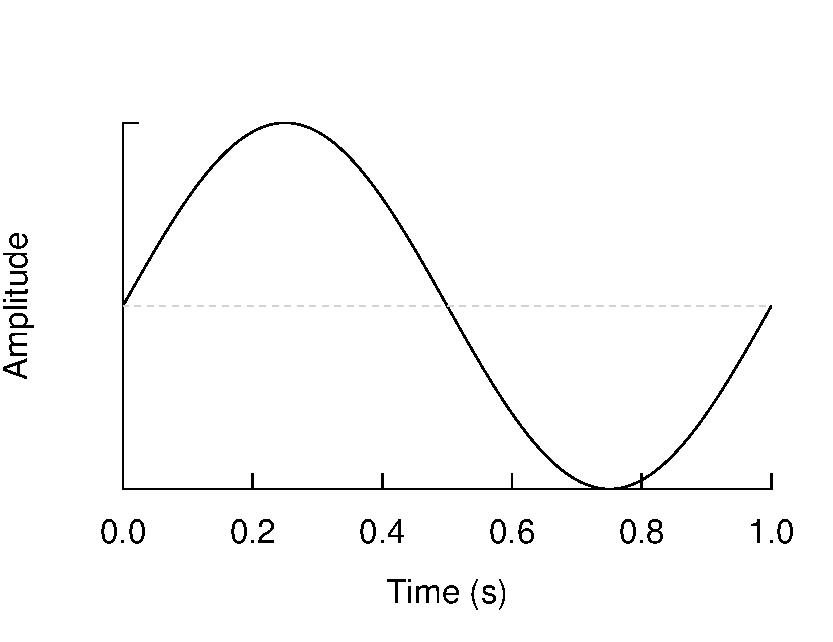
\includegraphics[width=196pt]{images/sine_full.pdf}
	\hspace{1em}
	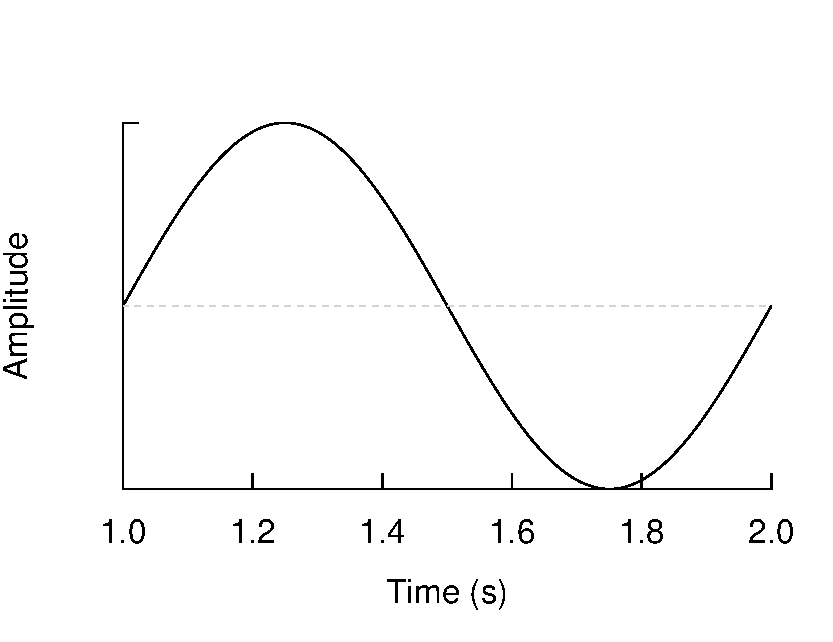
\includegraphics[width=196pt]{images/sine_shifted.pdf}
\end{figure}
\vspace{1em}
\begin{figure}[h]
\caption{Filtering/dilating a wavelet}\label{figure:filtering}
\caption*{\\[1em]\footnotesize\emph{Left: the input signal 1 second sine wave\\
Right:
the signal scaled to a 2 second sine wave}\rm}
\centering
	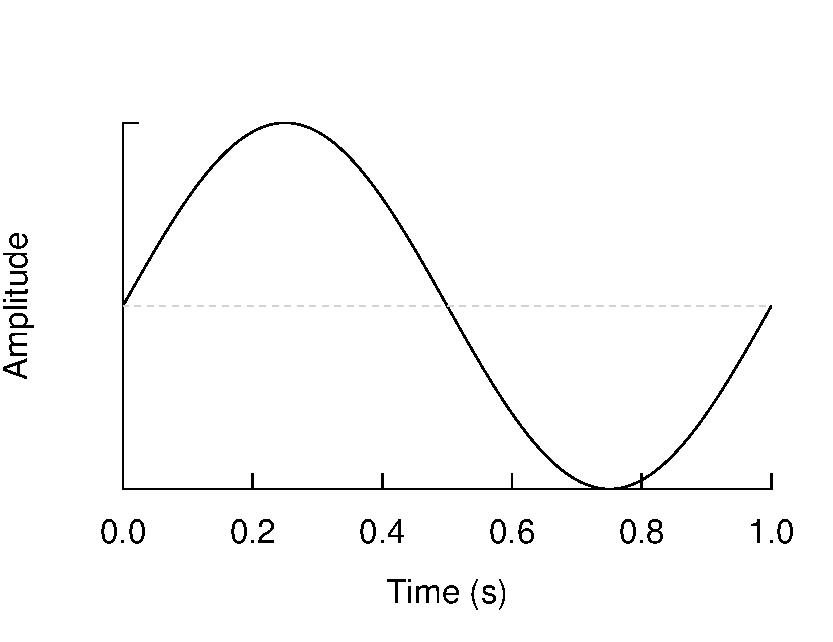
\includegraphics[width=196pt]{images/sine_full.pdf}
	\hspace{1em}
	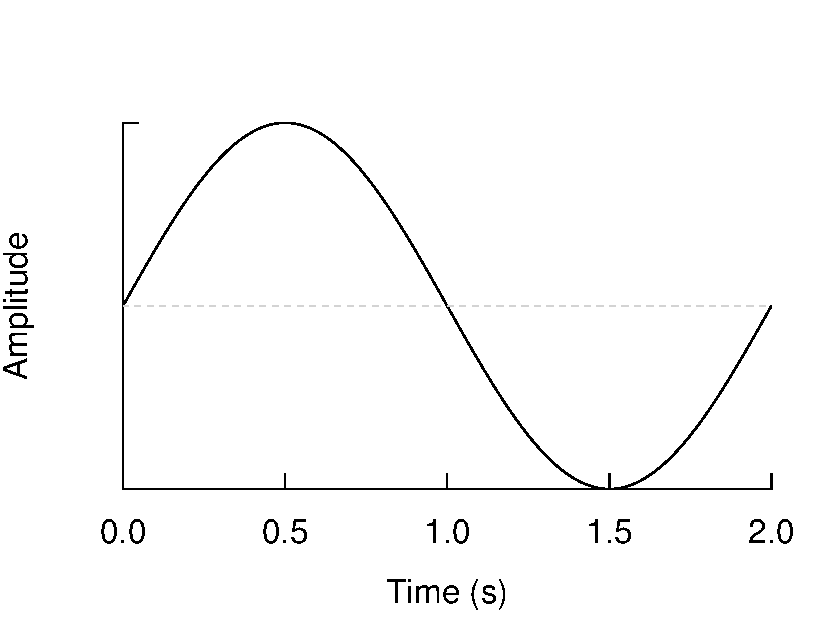
\includegraphics[width=196pt]{images/sine_scaled.pdf}
\end{figure}

\paragraph{}
Wavelet transform has proven to be important in signal processing thanks to its
inherent properties which allow comparisons at different scales and shifts
\cite{karus2013}. Compared to other time series analysis techniques, the main
advantages of wavelet transformations in the analysis of signals are:
\begin{itemize}
	\item Wavelet/shift coefficients allow fuzzy matching as differences in details
	are 'smoothed out'.
	\item Filter/scale coefficients allow detection of small anomalies in series.
	\item Decomposition levels make series of different lengths or scale
	comparable.
\end{itemize}

\subsection{Wavelet functions}
A wavelet function is a function that defines a wavelet \cite{wadkar}. Many
wavelet functions exist and differ largely in complexity and applicability
depending on the signal to be processed.

A wavelet can be defined in the following ways, given that $T$ is the set of
time values of the signal, and $F$ the set of frequency values of the signal 
\cite{graps}.
\begin{description}
	\item[Wavelet function (mother wavelet)] \hfill \\ $\Psi: T \rightarrow
	F$\\ $\Psi(t) = f$, such that $t \in T$ and $f \in F$.\\
	A bijective function mapping $T$ onto $F$ and producing the shape of the
	wavelet.

	\item[Scaling function (father wavelet)] \hfill \\ $\Phi: F \rightarrow
	T$\\ $\Phi(f) = t$, such that $t \in T$ and $f \in F$.\\
	A bijective function mapping $F$ onto $T$ and producing the scale of the
	wavelet.

	\item[Scaling filter] \hfill \\ A low-pass filter of length $2N$ and sum $1$.
	A high-pass filter can be calculated as the quadrature mirror filter of the
	low-pass filter. All Daubechies wavelets can be defined by the scaling filter.
\end{description}

\subsection{Haar wavelet}
The Haar wavelet is a member of the Daubechies family of wavelets, based on the
work of the Belgian mathematician Ingrid Daubechies \cite{graps}. The
Daubechies wavelets is a family of orthogonal wavelets defining a discrete
wavelet transform. All wavelets of the Daubechies family can be entirely
defined by their scaling filter.

The Haar wavelet is a Daubechies wavelet and has a filter length of 2 and
is therefore also referred to as the Daubechies-2 (D2) filter. It is the
simplest wavelet of the Daubechies family and is defined by the mother wavelet
function as shown in Figure \ref{figure:haar} \cite{stankovic}.

\begin{figure}[H]
\caption{The Haar functions}\label{figure:haar}
\centering
\caption*{\\[1em]\footnotesize\textit{(a) The Haar wavelet function (mother
wavelet)}}
\[
\begin{aligned}
\Psi(t) = \left\{
	\begin{array}{r r}
		1  & \quad   0 \leq t < 1/2, \\
		-1 & \quad 1/2 \leq t < 1, \\
		0  & \quad \text{otherwise.}
	\end{array}
\right.
\end{aligned}
\qquad
\raisebox{-15mm}{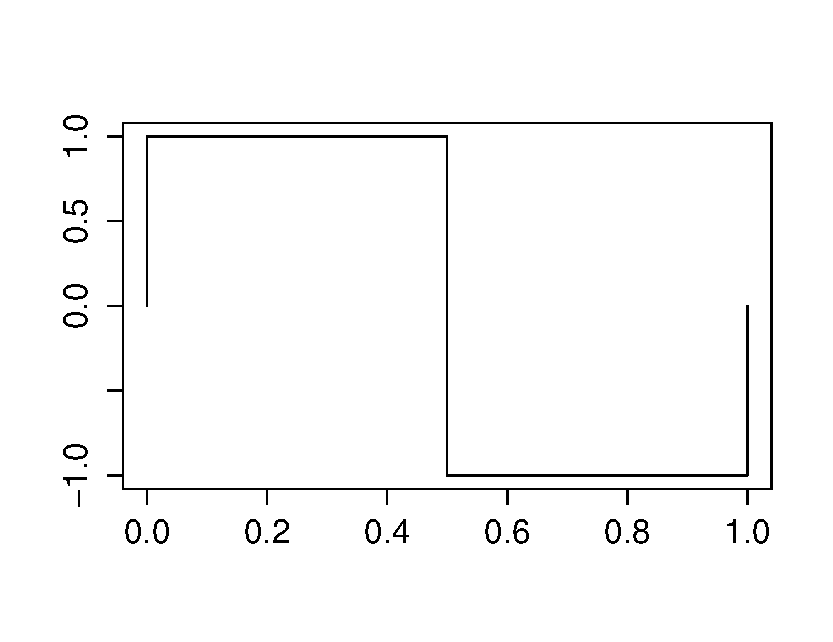
\includegraphics[height=128pt]{images/haar.pdf}}
\]
\caption*{\footnotesize\textit{(b) The Haar scaling function (father wavelet)}}
\[
\Phi(t) = \left\{
	\begin{array}{r r}
		1 & \quad 0 \leq t < 1, \\
		0 & \quad \text{otherwise.}
	\end{array}
\right.
\]
\end{figure}


\paragraph{}
In 1910, the Hungarian mathematician Alfred Haar introduced Haar functions. The
Haar transform is one of the earliest examples of what is known now as a
compact\footnote{Compact support: the ability of a function to be scaled
smoothly.}, dyadic\footnote{A dyadic function scales in powers of 2.},
orthonormal\footnote{Orthonormal: domain and range are orthogonal and of
equal length.} wavelet transform \cite{stankovic}. The Haar function is the
simplest and oldest orthonormal wavelet with compact support.

\subsection{Discrete Haar transform}
The Haar filter function varies in scale by splitting the input signal using
different scale sizes.

Having a signal over the domain from 0 to 1, the Haar transform divides the
signal into two wavelets that range from 0 to $1/2$ and from $1/2$ to 1. Then
the division can be repeated giving four wavelets that range from 0 to $1/4$,
from $1/4$ to $2/4$, from $2/4$ to $3/4$, and from $3/4$ to 1 \cite{graps}.

\paragraph{}
The original signal is decomposed successfully into components of lower
resolution. The decomposition can be repeated as long as the resolution of
the original signal allows. In the case of the Haar filter this means as long
as the number of resulting coefficients is larger than 2 (i.e., the filter
length).

\paragraph{}
In each scaling/filtering step (i.e., decomposition) the Haar function adds
more detail to the wavelets in the current level. The Haar filter captures the
differences between scale levels. These resulting coefficients can be used to
compare signals regardless of scale or length \cite{graps}.

Wavelet transform using the Haar filter is illustrated in Figure
\ref{figure:haar_transform}. The figure shows a stacked plot of a signal
(lower most graph) and the transformed signals at each level of decomposition
(the stack).

\begin{figure}[H]
\caption{Discrete wavelet transform using Haar
filter}\label{figure:haar_transform}
\caption*{\\[0em]\footnotesize\textit{$W1, \ldots, W6$ represent the levels of
decomposition in reversed order, the lower most graph shows the original
signal. The coefficients plotted at $W6$ (top most graph) are generated in the
first step of decomposing. Each level from $W6$ to $W1$ adds detail from the
original signal. The highest level ($W1$) is closest to the original signal. No
more detail is left from the original signal that can be added in any further
step.}\\[1em]}
\centering
	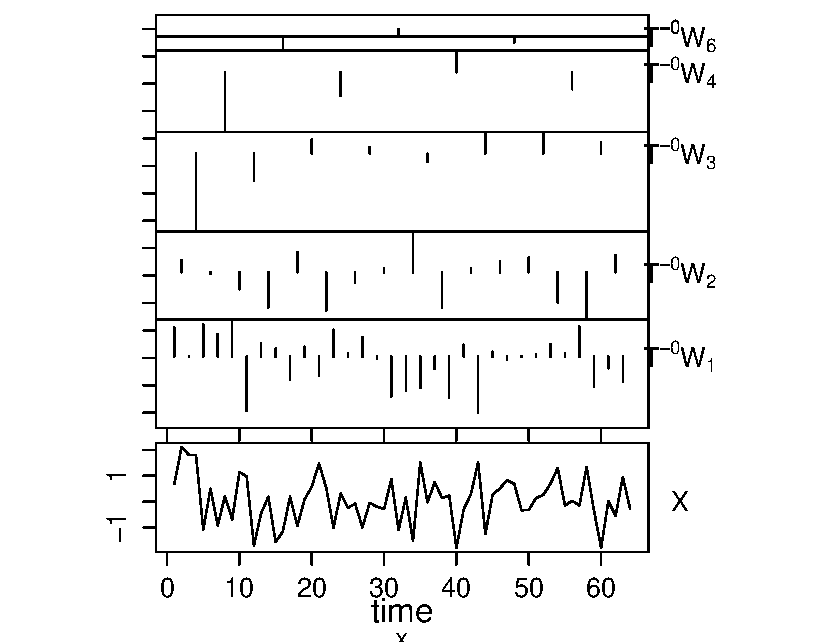
\includegraphics[scale=0.9]{images/dwt_haar.pdf}
\end{figure}

The spikes shown in Figure \ref{figure:haar_transform} represent the
coefficients found at the relevant level. The number of coefficients increases
by a factor of 2 at each level. In the figure, the original signal consists of
64 samples, therefore, the signal can be decomposed to a maximum of $64 \log_{2}
= 6$ levels.

\paragraph{}
The coefficients should only be compared to coefficients of the same type. The
scale/filter coefficients are incomparable to the wavelet/shift coefficients,
because that would mean comparing time with frequency which leads to invalid
relations between signals.

\paragraph{}
Wavelet transform using the Haar filter is widely used in other fields. For
example, as a way of digitalising an analogue signal in A-D converters, pattern
recognition in image and video processing, face recognition, image processing,
data coding, multiplexing, digital filtering, digital speech processing, voice
controlled computing devices, robotics, and compression mechanisms \cite{khan,
stankovic, wadkar}.

\begin{comment}
- Literature study
- Software evolution
- Project success
- Project survivability

This chapter contains all the information needed to put the thesis into
context. It is common to use (a revised version) of your literature survey for
this purpose.

It is important to refer from your text to sources you have used, as listed in
your bibliography section (appendix). For example, “XP is a recent agile
development method [1]” is a common style of doing this, where the following
entry would be included in your bibliography:
[1] K. Beck, E. Gamma, Test infected: Programmers love writing tests, Java
Report 3 (7) (1998) 51–56.

If you want to refer to books you have read as part of the curriculum, you can
also do so in this way.

Have a look at Chapter 2 of this example thesis at Paul’s
homepage\footnote{http://homepages.cwi.nl/~paulk/thesesMasterSoftwareEngineering/2006/RichardKettelerij.pdf}.
\end{comment}